\chapter{Functionele organisatie van de eukaryote cel}\label{ch:b1:eukaryotic-cell}

Een \omterm{def:b1:cell-unit-of-life:cell}{cel} van de alvleesklier maakt elke dag ongeveer haar eigen massa aan
verteringsenzymen en giet die in een afvoerbuis. Die enzymen zijn eiwitten die de
\omterm{def:b1:cell-unit-of-life:cell}{cel} die ze maakte zouden verteren; daarom bouwt de \omterm{def:b1:cell-unit-of-life:cell}{cel} ze binnen een afgesloten
membraanblad, verscheept ze door een tweede compartiment waar ze worden gesorteerd
en geconcentreerd, slaat ze op in korrels, en geeft ze pas vrij op het signaal
van een maaltijd. Elke stap gebeurt in een andere door membranen begrensde
ruimte, en het verkeer tussen die ruimten wordt door blaasjes verzorgd. Dit
hoofdstuk beschrijft de compartimenten van de \omterm{def:b1:cell-unit-of-life:prokeuk}{eukaryote cel}, het
\omterm{def:b1:eukaryotic-cell:endomembrane}{endomembraansysteem} waar de eiwitten doorheen stromen, de \omterm{def:b1:cell-unit-of-life:prokeuk}{organellen} die energie
omzetten, het skelet dat de vorm van de \omterm{def:b1:cell-unit-of-life:cell}{cel} bewaart en haar onderdelen verplaatst,
en de kenmerken die een plantencel van een dierlijke onderscheiden.

\section{Compartimenten}

\begin{definition}[Organel, cytosol]\label{def:b1:eukaryotic-cell:organelle}
Een \emph{organel}\index{organel} is een structuur binnen een \omterm{def:b1:cell-unit-of-life:cell}{cel} met een
bepaalde samenstelling en functie; de door membranen begrensde \omterm{def:b1:cell-unit-of-life:prokeuk}{organellen} zijn
compartimenten waarvan de inhoud in samenstelling verschilt van het
\emph{cytosol}\index{cytosol}, de waterige oplossing van het \omterm{def:b1:cell-unit-of-life:cell}{cytoplasma} daarbuiten.
Door membranen begrensde compartimenten: de \omterm{def:b1:eukaryotic-cell:nucleus}{celkern}, het \omterm{def:b1:eukaryotic-cell:endomembrane}{endoplasmatisch
reticulum}, het \omterm{def:b1:eukaryotic-cell:endomembrane}{golgi-apparaat}, de \omterm{def:b1:eukaryotic-cell:endomembrane}{lysosomen}, de \omterm{def:b1:eukaryotic-cell:peroxisome}{peroxisomen}, de \omterm{def:b1:eukaryotic-cell:mitochondrion}{mitochondriën}, en
bij planten de \omterm{def:b1:eukaryotic-cell:plastid}{plastiden} en de \omterm{def:b1:eukaryotic-cell:plantcell}{vacuole}. \omterm{def:b1:cell-unit-of-life:prokeuk}{Organellen} zonder membraan: de ribosomen,
het \omterm{def:b1:eukaryotic-cell:cytoskeleton}{centrosoom}, het \omterm{def:b1:eukaryotic-cell:cytoskeleton}{cytoskelet}.
\end{definition}

\begin{omfigure}
\begin{tikzpicture}
  \node[anchor=south west, inner sep=0] (img) at (0,0)
    {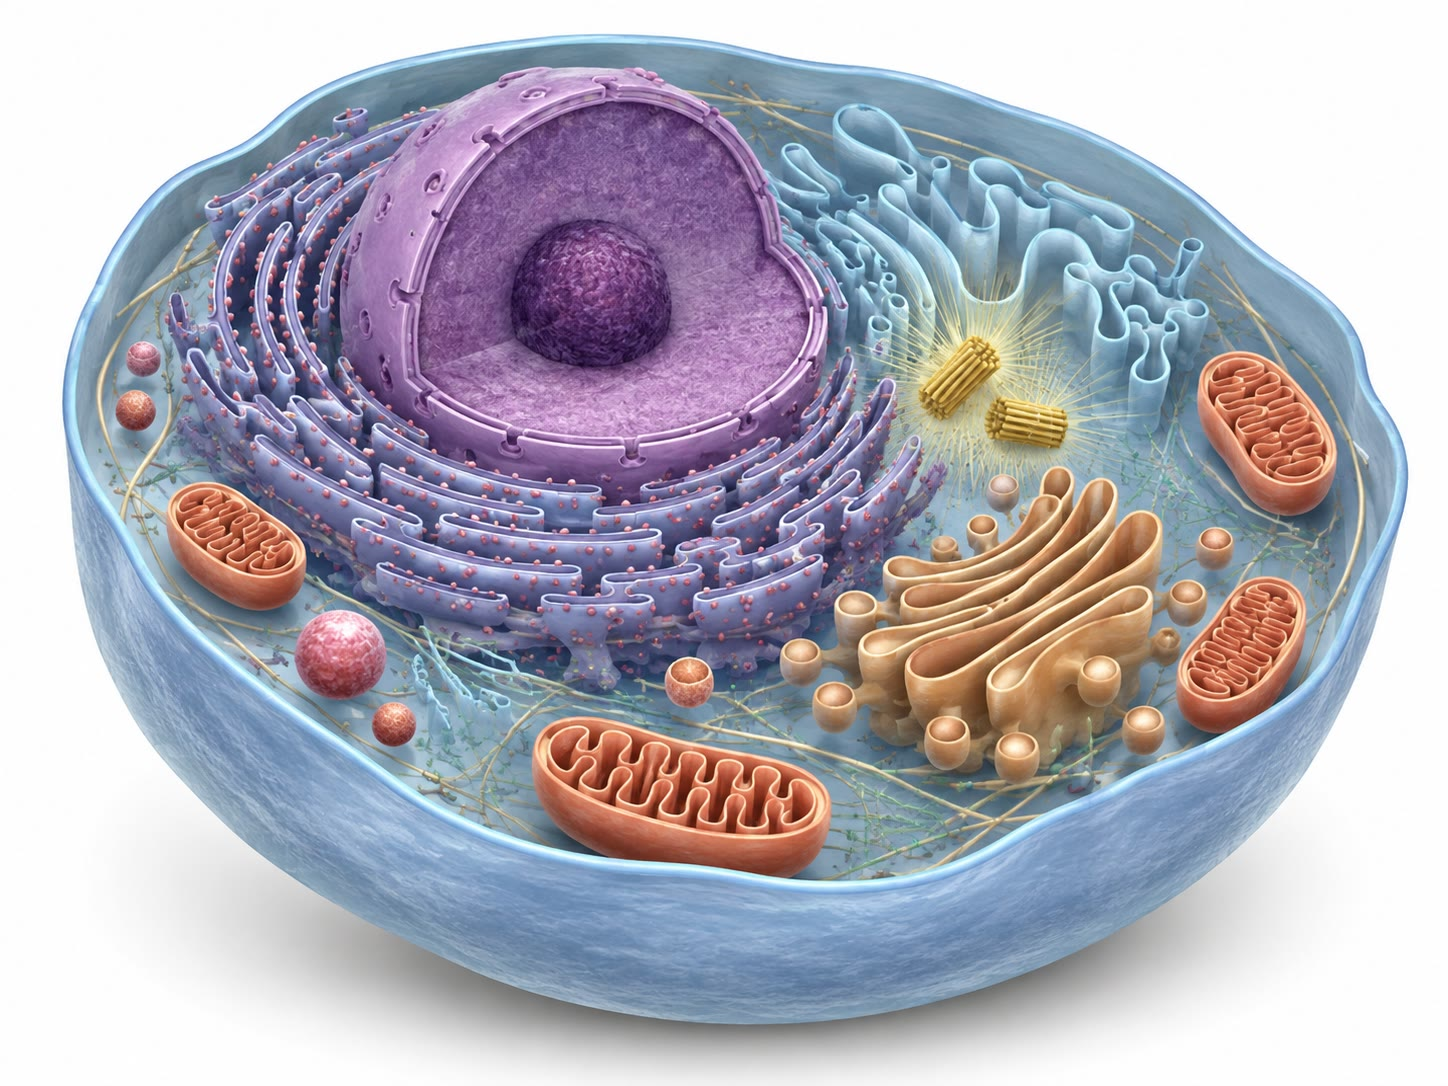
\includegraphics[width=0.6\linewidth]{images/book3/ai/fig-animal-cell-cutaway.jpg}};
  \begin{scope}[x={(img.south east)}, y={(img.north west)},
      every node/.style={font=\small}]
    \draw[omDef, thick] (0.42,0.72) -- (0.42,1.08) node[above] {celkern, nucleolus, poriën};
    \draw[omDef, thick] (0.30,0.52) -- (-0.03,0.44) node[left, align=right] {ruw endoplasmatisch\\ reticulum};
    \draw[omDef, thick] (0.23,0.42) -- (-0.03,0.22) node[left] {lysosoom};
    \draw[omDef, thick] (0.07,0.62) -- (-0.03,0.76) node[left] {plasmamembraan};
    \draw[omDef, thick] (0.75,0.80) -- (1.03,0.88) node[right] {glad ER};
    \draw[omDef, thick] (0.69,0.63) -- (1.03,0.62) node[right] {centrosoom};
    \draw[omDef, thick] (0.87,0.42) -- (1.03,0.36) node[right] {mitochondrion};
    \draw[omDef, thick] (0.70,0.40) -- (0.80,-0.08) node[below] {golgi-apparaat en blaasjes};
    \draw[omDef, thick] (0.47,0.25) -- (0.35,-0.08) node[below] {mitochondrion};
  \end{scope}
\end{tikzpicture}

{\small Een algemene dierlijke \omterm{def:b1:cell-unit-of-life:cell}{cel}, opengesneden. De \omterm{def:b1:eukaryotic-cell:nucleus}{celkern} in het midden;
daaromheen het \omterm{def:b1:eukaryotic-cell:endomembrane}{ruwe} \omterm{def:b1:eukaryotic-cell:endomembrane}{endoplasmatisch reticulum} dat overgaat in de \omterm{def:b1:eukaryotic-cell:nucleus}{kernenvelop}, het
\omterm{def:b1:eukaryotic-cell:endomembrane}{gladde} reticulum, de golgistapel met haar blaasjes, \omterm{def:b1:eukaryotic-cell:mitochondrion}{mitochondriën}, \omterm{def:b1:eukaryotic-cell:endomembrane}{lysosomen}, en
het \omterm{def:b1:eukaryotic-cell:cytoskeleton}{centrosoom} van waaruit de \omterm{def:b1:eukaryotic-cell:cytoskeleton}{microtubuli} stralen.}
\end{omfigure}

\begin{definition}[De celkern]\label{def:b1:eukaryotic-cell:nucleus}
De \emph{celkern}\index{celkern} bevat de chromosomen als
\emph{chromatine}\index{chromatine}, DNA gewonden om histoneiwitten
(\cref{ch:b1:genomes}). Zij is begrensd door de
\emph{kernenvelop}\index{kernenvelop}, twee membranen waarvan de buitenste
overgaat in het \omterm{def:b1:eukaryotic-cell:endomembrane}{endoplasmatisch reticulum}, doorboord door
\emph{kernporiën}\index{kernporie} waardoor RNA en eiwitten in beide richtingen
gecontroleerd passeren. De \emph{nucleolus}\index{nucleolus} is het gebied waar
ribosomaal RNA wordt gemaakt en ribosomen worden gebouwd. De celkern scheidt de
transcriptie (binnen) van de translatie (buiten), een scheiding die prokaryoten
niet kennen.
\end{definition}

\begin{proposition}[De compartimenten van een levercel]\label{prop:b1:eukaryotic-cell:budget}
In een hepatocyt van \qty{5000}{\micro m^3} neemt het \omterm{def:b1:eukaryotic-cell:organelle}{cytosol} ongeveer de helft
van het volume in, de \omterm{def:b1:eukaryotic-cell:mitochondrion}{mitochondriën} een vijfde, het \omterm{def:b1:eukaryotic-cell:endomembrane}{endoplasmatisch reticulum} een
zesde, de \omterm{def:b1:eukaryotic-cell:nucleus}{celkern} een zestiende, en het \omterm{def:b1:eukaryotic-cell:endomembrane}{golgi-apparaat}, de \omterm{def:b1:eukaryotic-cell:endomembrane}{lysosomen} en de
\omterm{def:b1:eukaryotic-cell:peroxisome}{peroxisomen} samen enkele procenten. De membranen vertellen een ander verhaal: van
de \qty{110000}{\micro m^2} membraan in de \omterm{def:b1:cell-unit-of-life:cell}{cel} is de helft \omterm{def:b1:eukaryotic-cell:endomembrane}{endoplasmatisch
reticulum}, een derde het binnenmembraan van de \omterm{def:b1:eukaryotic-cell:mitochondrion}{mitochondriën}, en slechts
\qty{2}{\%} de plasmamembraan. Het meeste membraan van een \omterm{def:b1:cell-unit-of-life:cell}{cel} zit binnenin.
\end{proposition}

\begin{omfigure}
\begin{tikzpicture}
\begin{axis}[
  xbar, bar width=8pt,
  width=0.72\linewidth, height=6.4cm,
  axis x line=bottom, axis y line=left,
  xmin=0, xmax=45, xlabel={aandeel in het totale membraan van de cel (\%)},
  xlabel style={font=\small, at={(axis description cs:0.5,-0.13)}, anchor=north},
  symbolic y coords={kernenvelop, plasmamembraan, lysosomen en peroxisomen, golgi-apparaat, buitenmembraan mitochondrion, glad ER, binnenmembraan mitochondrion, ruw ER},
  ytick=data, tick label style={font=\small},
  enlarge y limits=0.08, xtick={0,10,20,30,40},
  nodes near coords, nodes near coords style={font=\scriptsize, anchor=west},
]
\addplot[fill=omDef!45, draw=omDef] coordinates
  {(0.2,kernenvelop) (2,plasmamembraan) (1.5,lysosomen en peroxisomen) (7,golgi-apparaat) (7,buitenmembraan mitochondrion) (16,glad ER) (32,binnenmembraan mitochondrion) (35,ruw ER)};
\end{axis}
\end{tikzpicture}

{\small Waar het membraan van een levercel zit. De plasmamembraan, de enige die
van buitenaf zichtbaar is, is twee procent van het totaal; het reticulum en het
binnenmembraan van de \omterm{def:b1:eukaryotic-cell:mitochondrion}{mitochondriën}, binnenin opgevouwen, zijn vier vijfde.}
\end{omfigure}

\section{Het endomembraansysteem}

\begin{definition}[Endoplasmatisch reticulum, golgi-apparaat, lysosoom]\label{def:b1:eukaryotic-cell:endomembrane}
Het \emph{endoplasmatisch reticulum}\index{endoplasmatisch reticulum} (ER) is een
netwerk van membraanbladen en buizen dat één aaneengesloten ruimte omsluit, het
lumen, en overgaat in de \omterm{def:b1:eukaryotic-cell:nucleus}{kernenvelop}. Het
\emph{ruwe}\index{ruw endoplasmatisch reticulum} deel is bezet met ribosomen die
de eiwitten die zij maken het lumen of de membraan in duwen; het
\emph{gladde}\index{glad endoplasmatisch reticulum} deel maakt lipiden, slaat
calcium op en ontgift. Het \emph{golgi-apparaat}\index{golgi-apparaat} is een
stapel afgeplatte zakjes (cisternen), met een ontvangende \emph{cis}-zijde bij het
ER en een verzendende \emph{trans}-zijde, waarin eiwitten uit het ER worden
gewijzigd (suikers bijgesneden en toegevoegd), gesorteerd, en in blaasjes verpakt
voor hun bestemming. \emph{Lysosomen}\index{lysosoom} zijn zure blaasjes (pH
$\approx 5$) vol hydrolytische enzymen die van buiten aangevoerd materiaal of
versleten \omterm{def:b1:cell-unit-of-life:prokeuk}{organellen} verteren. Samen met de blaasjes die tussen hen en de
plasmamembraan heen en weer gaan, vormen zij het
\emph{endomembraansysteem}\index{endomembraansysteem}: één samenhangend stel
compartimenten waarvan de lumina topologisch de buitenkant van de \omterm{def:b1:cell-unit-of-life:cell}{cel} zijn.
\end{definition}

\begin{proposition}[De secretieroute]\label{prop:b1:eukaryotic-cell:secretory}
\index{secretieroute}
Een eiwit dat bestemd is voor afscheiding, voor de plasmamembraan of voor een
\omterm{def:b1:eukaryotic-cell:endomembrane}{lysosoom} wordt gemaakt door ribosomen die aan het \omterm{def:b1:eukaryotic-cell:endomembrane}{ruwe} ER gebonden zijn, komt
tijdens zijn synthese het ER-lumen binnen, vouwt zich daar, reist in blaasjes naar
de cis-zijde van het \omterm{def:b1:eukaryotic-cell:endomembrane}{golgi-apparaat}, doorkruist de stapel terwijl het wordt
gewijzigd, en verlaat de trans-zijde in een blaasje dat aan zijn bestemming is
geadresseerd: een secretiekorrel die op een signaal met de plasmamembraan
versmelt (\emph{gereguleerde exocytose}\index{exocytose}), een blaasje dat
onafgebroken versmelt (\emph{constitutieve} exocytose, die tevens nieuw membraan
aanvoert), of een \omterm{def:b1:eukaryotic-cell:endomembrane}{lysosoom}. Cytosolische en kerneiwitten worden op vrije
ribosomen gemaakt en komen het systeem nooit binnen. Wat beslist, is een
\emph{signaalsequentie}\index{signaalsequentie} aan het begin van het eiwit
(\cref{ch:b1:gene-expression}).
\end{proposition}
\begin{proof}[Bewijsmateriaal]
Palade (jaren 1960) gaf plakjes cavia-alvleesklier drie minuten lang radioactieve
aminozuren (de \emph{puls}), daarna ongemerkte (de \emph{jacht}), en lokaliseerde
de radioactiviteit met autoradiografie van elektronenmicroscopische opnamen op
gezette tijden. Na \qty{3}{min} lagen de zilverkorrels boven het \omterm{def:b1:eukaryotic-cell:endomembrane}{ruwe} ER; na
\qty{20}{min} boven het \omterm{def:b1:eukaryotic-cell:endomembrane}{golgi-apparaat}; na \qty{40}{min} boven condenserende
\omterm{def:b1:eukaryotic-cell:plantcell}{vacuolen} en nieuwe korrels; na \qty{2}{h} in het lumen van de afvoerbuis.
\omterm{def:b1:cell-unit-of-life:fractionation}{Celfractionering} gaf langs chemische weg dezelfde volgorde. Blobel (jaren 1970)
toonde aan dat secretie-eiwitten die in een reageerbuis zonder membranen worden
gemaakt twintig residuen langer zijn dan de afgescheiden vorm en niet tegen een
toegevoegd protease beschermd zijn, terwijl zij bij aanwezigheid van
ER-membranen wel worden geknipt en beschermd: de extra residuen zijn het signaal
dat de groeiende keten het ER in stuurt.
\end{proof}

\begin{omfigure}
\begin{tikzpicture}
\begin{axis}[
  width=0.9\linewidth, height=6.2cm,
  axis x line=bottom, axis y line=left,
  xmin=0, xmax=130, ymin=0, ymax=105,
  xlabel={tijd na de puls (min)}, ylabel={aandeel van het merk (\%)},
  xlabel style={font=\small, at={(axis description cs:0.5,-0.12)}, anchor=north},
  ylabel style={font=\small},
  tick label style={font=\small}, xtick={0,20,40,60,80,100,120}, ytick={0,25,50,75,100},
  legend style={font=\small, at={(0.5,-0.24)}, anchor=north, draw=none, legend columns=2, /tikz/every even column/.append style={column sep=0.4cm}},
  clip=false,
]
\addplot[very thick, omDef, smooth] coordinates {(3,88) (7,55) (15,25) (30,8) (60,2) (120,0)};
\addlegendentry{ruw ER}
\addplot[very thick, omProp, smooth] coordinates {(3,8) (7,35) (15,55) (30,35) (60,10) (120,2)};
\addlegendentry{golgi-apparaat en condenserende vacuolen}
\addplot[very thick, omThm, smooth] coordinates {(3,0) (7,3) (15,12) (30,45) (60,70) (90,55) (120,30)};
\addlegendentry{secretiekorrels}
\addplot[very thick, omExo, smooth] coordinates {(3,0) (7,0) (15,0) (30,2) (60,12) (90,35) (120,65)};
\addlegendentry{afgescheiden in de afvoerbuis}
\end{axis}
\end{tikzpicture}

{\small De puls-jachtproef van Palade in de alvleesklier: waar de gemerkte
eiwitten zich bevinden als functie van de tijd. Zij gaan in een kwartier van het
ER naar het \omterm{def:b1:eukaryotic-cell:endomembrane}{golgi-apparaat}, bereiken de korrels binnen het uur, en verlaten de
\omterm{def:b1:cell-unit-of-life:cell}{cel} in de twee uur daarna.}
\end{omfigure}

\begin{omfigure}
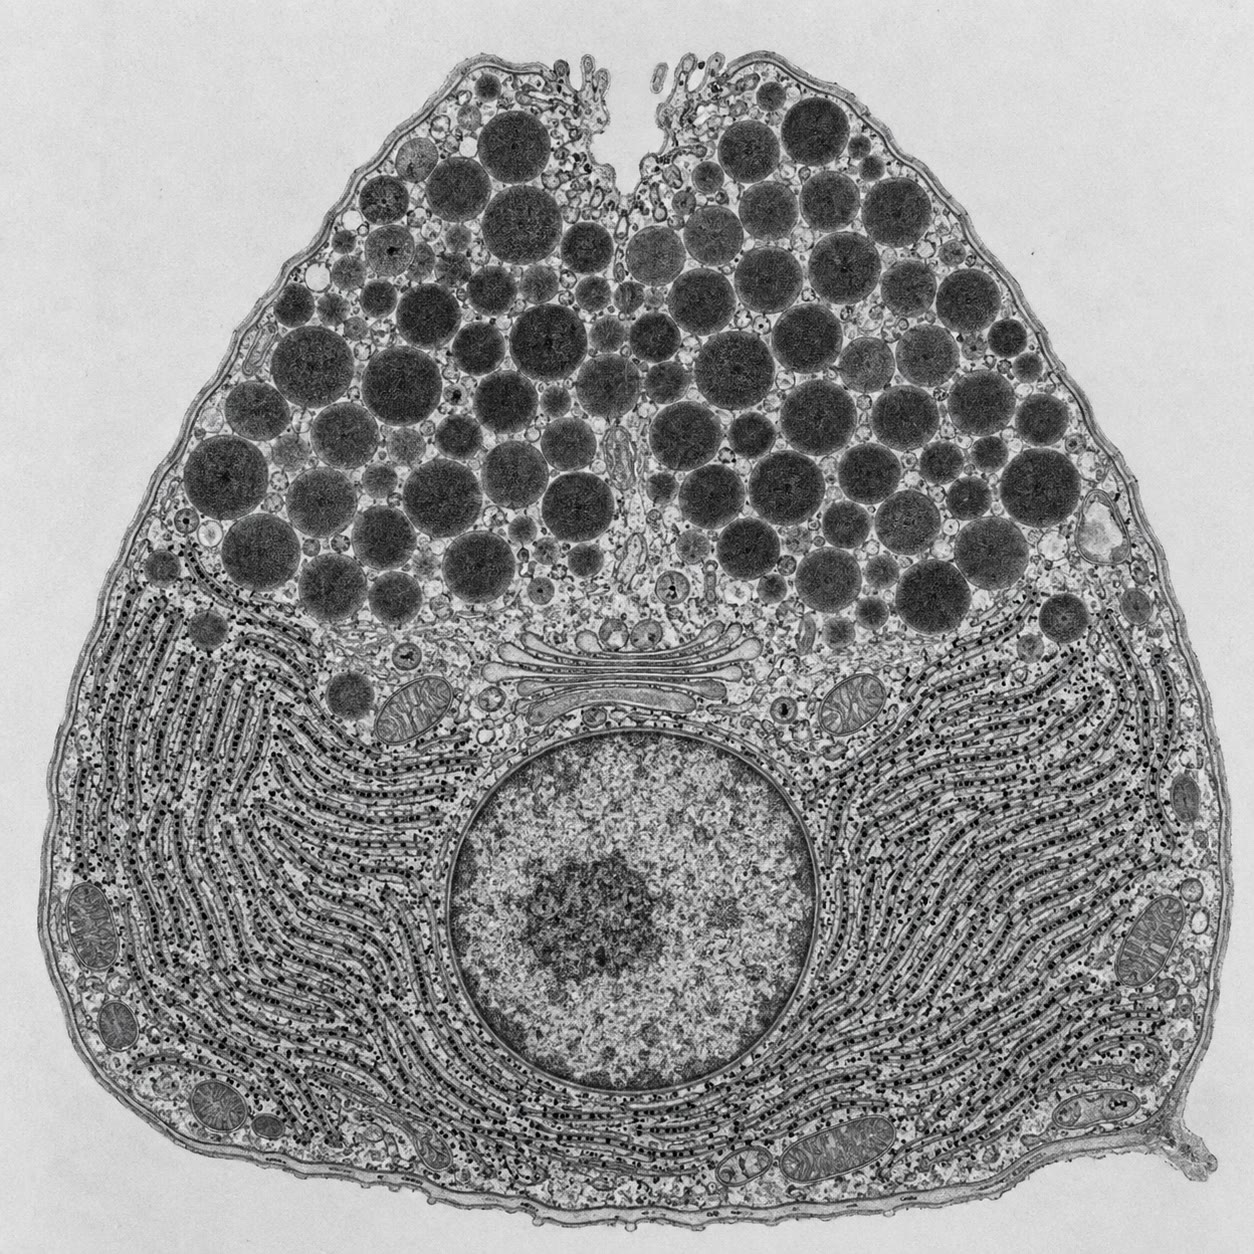
\includegraphics[width=0.44\linewidth]{images/book3/ai/b3-06-acinar-cell-tem.jpg}

{\small Een acinaire \omterm{def:b1:cell-unit-of-life:cell}{cel} van de alvleesklier in de
\omterm{prop:b1:cell-unit-of-life:microscopes}{transmissie-elektronenmicroscoop}: ruw ER in evenwijdige stapels rond de \omterm{def:b1:eukaryotic-cell:nucleus}{celkern}
aan de basis, het \omterm{def:b1:eukaryotic-cell:endomembrane}{golgi-apparaat} erboven, en de dichte secretiekorrels
opeengepakt naar de top en de afvoerbuis toe.}
\end{omfigure}

\begin{method}[Een molecuul door de cel volgen]\label{met:b1:eukaryotic-cell:pulsechase}
\begin{enumerate}
  \item Merk een korte lichting: stel de \omterm{def:b1:cell-unit-of-life:cell}{cellen} enkele minuten bloot aan
        een radioactieve of fluorescerende voorloper (de puls) en vervang
        die dan door een overmaat ongemerkte voorloper (de jacht), zodat
        alleen moleculen die tijdens de puls zijn gemaakt het merk dragen.
  \item Neem op gezette tijden monsters, fixeer, en lokaliseer het merk:
        met autoradiografie van coupes, met fluorescentiemicroscopie, of
        door fractionering en tellen.
  \item Het compartiment waarvan het merk het eerst piekt ligt
        stroomopwaarts; de volgorde van de pieken is de route; de tussen\-tijden
        zijn de transporttijden.
  \item Blokkeer een stap (kou, een energieremmer, een mutant) en kijk waar
        het merk zich ophoopt: in het compartiment vóór de blokkade.
\end{enumerate}
\end{method}

\begin{definition}[Endocytose]\label{def:b1:eukaryotic-cell:endocytosis}
\emph{Endocytose}\index{endocytose} brengt materiaal naar binnen: de
plasmamembraan stulpt eromheen naar binnen en snoert een blaasje af, dat
gewoonlijk met een \omterm{def:b1:eukaryotic-cell:endomembrane}{lysosoom} versmelt. \emph{Fagocytose} slokt deeltjes op (een
bacterie, een dode \omterm{def:b1:cell-unit-of-life:cell}{cel}); \emph{pinocytose} neemt druppeltjes vloeistof op;
\emph{receptorgemedieerde endocytose} concentreert een bepaald molecuul
(cholesteroldragende deeltjes, ijzerdragend transferrine) op receptoren in
beklede putjes voordat het wordt opgenomen. Exocytose voegt membraan aan het
celoppervlak toe en endocytose neemt het weg; in een afscheidende \omterm{def:b1:cell-unit-of-life:cell}{cel} houden de
twee elkaar in evenwicht, zodat het oppervlak constant blijft terwijl er elk uur
hele stukken membraan doorheen circuleren.
\end{definition}

\section{Mitochondriën en plastiden}

\begin{definition}[Mitochondrion]\label{def:b1:eukaryotic-cell:mitochondrion}
Een \emph{mitochondrion}\index{mitochondrion} is een \omterm{def:b1:eukaryotic-cell:organelle}{organel} van
\qtyrange{0.5}{1}{\micro m} dik en enkele micrometers lang, begrensd door twee
membranen: een glad buitenmembraan dat doorlaatbaar is voor kleine moleculen, en
een binnenmembraan dat tot \emph{cristae}\index{crista} is gevouwen, ondoorlaatbaar
is voor ionen en de ademhalingsketen en het ATP-synthase draagt
(\cref{ch:b1:respiration-fermentation}). Binnenin ligt de
\emph{matrix}\index{mitochondriale matrix}, met de enzymen van de krebscyclus,
ribosomen van het bacteriële type en verscheidene kopieën van een klein ringvormig
DNA. Mitochondriën delen door splitsing, bewegen langs het \omterm{def:b1:eukaryotic-cell:cytoskeleton}{cytoskelet}, en komen
per \omterm{def:b1:cell-unit-of-life:cell}{cel} in aantallen van enkele honderden tot enkele duizenden voor.
\end{definition}

\begin{definition}[Plastiden]\label{def:b1:eukaryotic-cell:plastid}
\emph{Plastiden}\index{plastide} zijn de \omterm{def:b1:cell-unit-of-life:prokeuk}{organellen} met een dubbele membraan van
plantencellen: \emph{chloroplasten}\index{chloroplast}, waarin een derde
membraanstelsel, de \emph{thylakoïden}\index{thylakoïde}, gestapeld tot grana en
gebaad in het \emph{stroma}\index{stroma}, de fotosynthese uitvoert
(\cref{ch:b1:photosynthesis}); amyloplasten, die zetmeel opslaan; chromoplasten,
die de kleurstoffen van vruchten en kroonbladen bevatten. Alle komen voort uit
proplastiden en bevatten, net als de \omterm{def:b1:eukaryotic-cell:mitochondrion}{mitochondriën}, hun eigen ringvormige DNA en
ribosomen van het bacteriële type, en delen door splitsing.
\end{definition}

\begin{omfigure}
\begin{minipage}[b]{0.48\linewidth}\centering
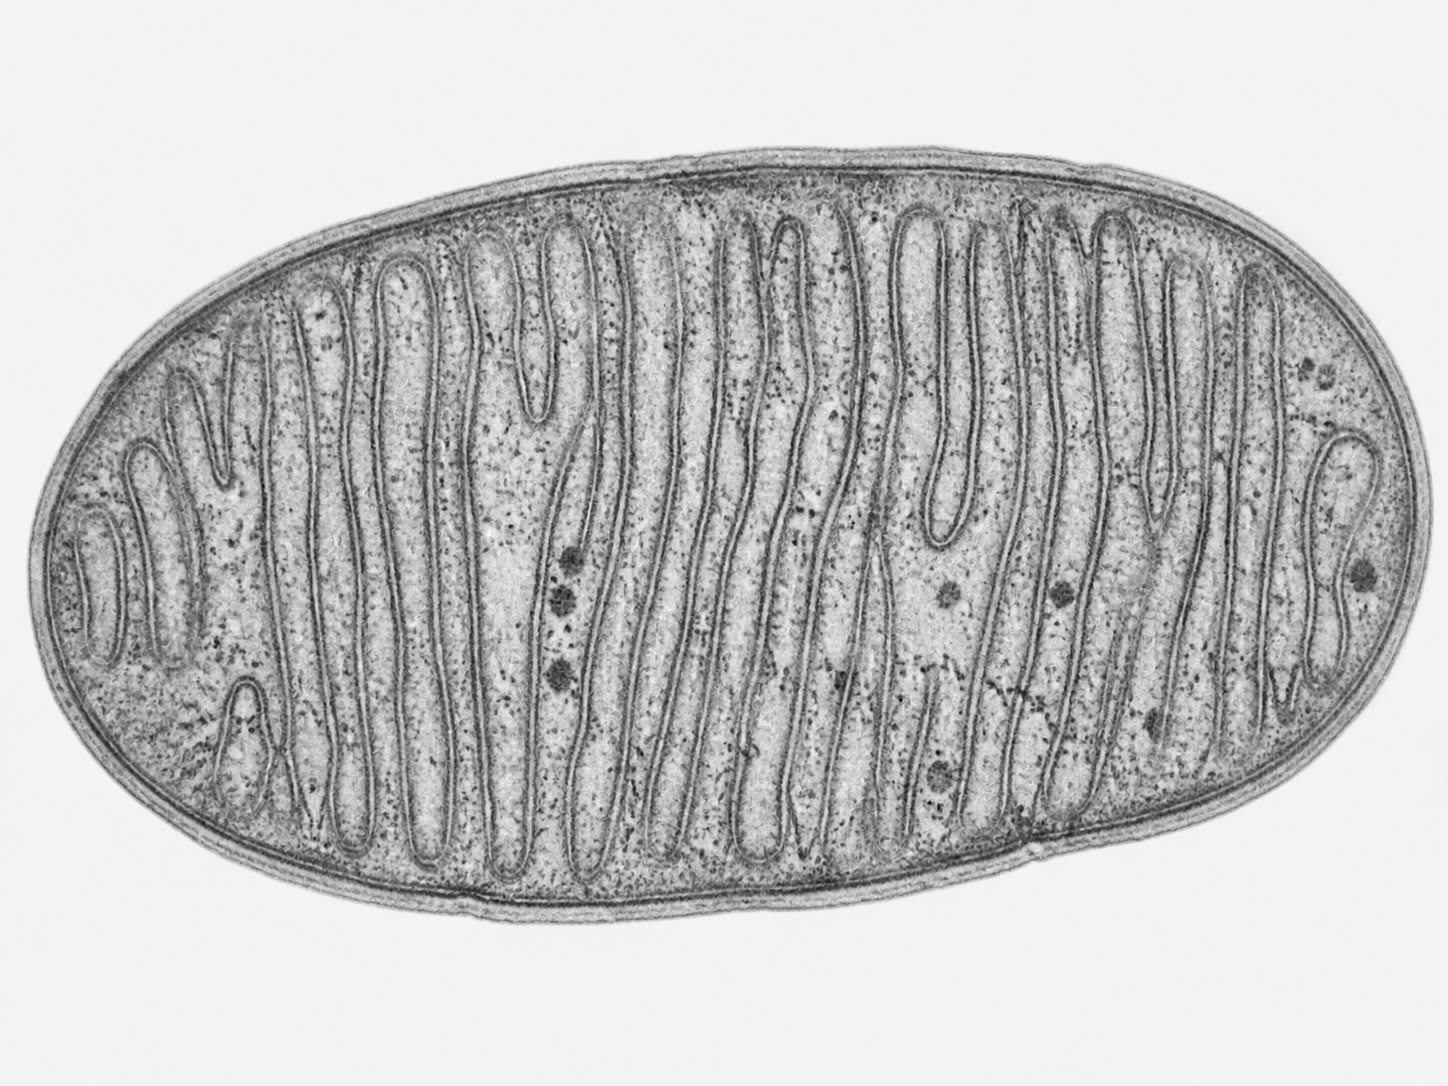
\includegraphics[width=0.96\linewidth]{images/book2/ai/g12-resp-mitochondrion-tem.jpg}
\end{minipage}\hfill
\begin{minipage}[b]{0.48\linewidth}\centering
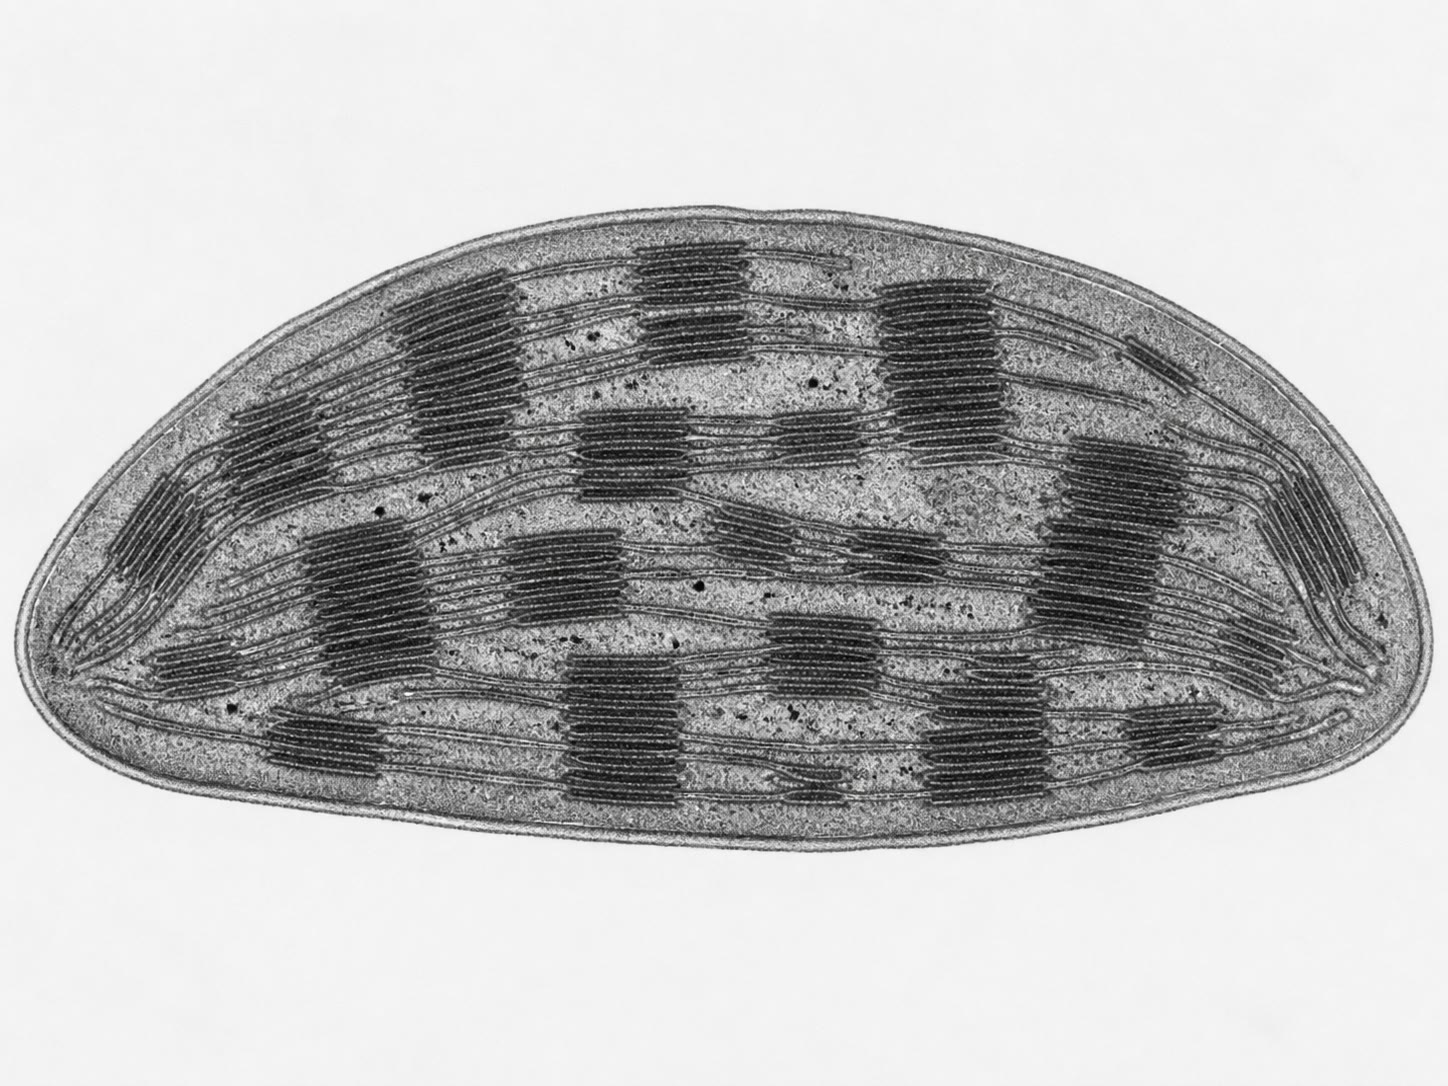
\includegraphics[width=0.96\linewidth]{images/book2/ai/g12-photo-chloroplast-tem.jpg}
\end{minipage}

{\small Een \omterm{def:b1:eukaryotic-cell:mitochondrion}{mitochondrion} (links) en een \omterm{def:b1:eukaryotic-cell:plastid}{chloroplast} (rechts) in doorsnede onder
de \omterm{prop:b1:cell-unit-of-life:microscopes}{elektronenmicroscoop}. Elk twee envelopmembranen; binnenin het gevouwen
binnenmembraan van het \omterm{def:b1:eukaryotic-cell:mitochondrion}{mitochondrion} en de gestapelde \omterm{def:b1:eukaryotic-cell:plastid}{thylakoïden} van de
\omterm{def:b1:eukaryotic-cell:plastid}{chloroplast} --- de membranen waarop energie wordt omgezet.}
\end{omfigure}

\begin{proposition}[Endosymbiotische oorsprong]\label{prop:b1:eukaryotic-cell:endosymbiosis}
\index{endosymbiose}
\omterm{def:b1:eukaryotic-cell:mitochondrion}{Mitochondriën} en \omterm{def:b1:eukaryotic-cell:plastid}{plastiden} stammen af van vrijlevende bacteriën die door een
voorouderlijke \omterm{def:b1:cell-unit-of-life:prokeuk}{eukaryote cel} zijn opgeslokt en als symbionten behouden:
\omterm{def:b1:eukaryotic-cell:mitochondrion}{mitochondriën} van een aerobe bacterie, \omterm{def:b1:eukaryotic-cell:plastid}{plastiden} van een cyanobacterie.
\end{proposition}
\begin{proof}[Bewijsmateriaal]
Beide \omterm{def:b1:cell-unit-of-life:prokeuk}{organellen} hebben twee membranen, waarvan het binnenste van bacteriële
samenstelling is en het buitenste op dat van de gastheer lijkt; een ringvormig
chromosoom zonder histonen; ribosomen van bacteriële afmeting en gevoeligheid voor
antibiotica; een genetische code met bacteriële varianten; deling door tweedeling
onafhankelijk van die van de \omterm{def:b1:cell-unit-of-life:cell}{cel}; en hun genen groeperen zich, eenmaal gesequencet,
bij die van bepaalde bacteriële lijnen (alfaproteobacteriën, cyanobacteriën) en
niet bij de kerngenen van de \omterm{def:b1:cell-unit-of-life:cell}{cel} die hen huisvest. De meeste van hun
oorspronkelijke genen zijn sindsdien naar de kern verhuisd, en de \omterm{def:b1:cell-unit-of-life:prokeuk}{organellen}
kunnen niet meer alleen leven.
\end{proof}

\begin{definition}[Peroxisoom]\label{def:b1:eukaryotic-cell:peroxisome}
Een \emph{peroxisoom}\index{peroxisoom} is een klein \omterm{def:b1:eukaryotic-cell:organelle}{organel} met één membraan dat
oxidatieve enzymen bevat die waterstof van substraten (vetzuren, alcohol) op
zuurstof overdragen, waarbij waterstofperoxide ontstaat, en katalase, dat het
peroxide ter plaatse afbreekt. Het sluit een gevaarlijke chemie op.
\end{definition}

\section{Het cytoskelet}

\begin{definition}[Cytoskelet]\label{def:b1:eukaryotic-cell:cytoskeleton}
Het \emph{cytoskelet}\index{cytoskelet} is een netwerk van eiwitfilamenten dat de
\omterm{def:b1:cell-unit-of-life:cell}{cel} haar vorm geeft, haar \omterm{def:b1:cell-unit-of-life:prokeuk}{organellen} verankert, en die \omterm{def:b1:cell-unit-of-life:prokeuk}{organellen} en de \omterm{def:b1:cell-unit-of-life:cell}{cel} zelf
verplaatst. Er zijn drie typen:
\emph{microfilamenten}\index{microfilament} van actine (\qty{7}{nm}, twee
gedraaide strengen bolvormige eenheden), geconcentreerd onder de plasmamembraan
en verantwoordelijk voor de celvorm, het kruipen, de contractiele ring van de
deling en de spiercontractie met myosine;
\emph{microtubuli}\index{microtubulus} (holle buizen van \qty{25}{nm} uit
tubuline), die uitstralen vanuit het \emph{centrosoom}\index{centrosoom}, sporen
waarlangs motoreiwitten (kinesine naar buiten, dyneïne naar binnen) blaasjes en
\omterm{def:b1:cell-unit-of-life:prokeuk}{organellen} vervoeren, de spoelfiguur van de deling, en de kern van trilharen en
zweepstaarten; \emph{intermediaire filamenten}\index{intermediair filament}
(\qty{10}{nm}, touwachtig, van keratines en verwante eiwitten), de mechanisch
sterke vezels die \omterm{def:b1:cell-unit-of-life:cell}{cellen} verstevigen en aan desmosomen verankeren.
Microfilamenten en microtubuli worden voortdurend uit hun voorraad bouwstenen
opgebouwd en weer afgebroken.
\end{definition}

\begin{omfigure}
\begin{tikzpicture}[font=\footnotesize, line cap=round]
  % actin: two twisted strands of beads
  \foreach \i in {0,...,15} {
    \pgfmathsetmacro{\y}{0.13*sin(\i*45)}
    \fill[omThm!70] (0.35*\i,1.6+\y) circle (0.11);
    \fill[omThm!45] (0.35*\i+0.17,1.6-\y) circle (0.11);
  }
  \node[anchor=west, align=left] at (6.0,1.6) {\textbf{microfilament} (actine), \qty{7}{nm}\\ vorm, kruipen, delingsring, spier};
  % intermediate filament: rope of coiled strands
  \foreach \k in {0,1,2,3} {
    \draw[omProp, thick] plot[domain=0:5.3, samples=60] (\x, {0.55+0.09*sin(180*\x+90*\k)});
  }
  \node[anchor=west, align=left] at (6.0,0.55) {\textbf{intermediair filament}, \qty{10}{nm}\\ touwachtig, mechanische sterkte};
  % microtubule: hollow tube of protofilaments
  \draw[thick, omDef!70!black, fill=omDef!15] (0,-0.9) rectangle (5.3,-0.2);
  \foreach \i in {0,...,25} { \foreach \j in {0,1,2,3} {
    \fill[omDef!60] (0.1+0.2*\i, -0.83+0.19*\j) circle (0.075);
  } }
  \draw[thick, omDef!70!black, fill=omDef!10] (5.3,-0.55) ellipse (0.18 and 0.35);
  \draw[thick, omDef!70!black, fill=white] (5.3,-0.55) ellipse (0.10 and 0.24);
  \node[anchor=west, align=left] at (6.0,-0.55) {\textbf{microtubulus} (tubuline), \qty{25}{nm} hol\\ sporen voor motoren, spoelfiguur, trilharen};
\end{tikzpicture}

{\small De drie filamenten van het \omterm{def:b1:eukaryotic-cell:cytoskeleton}{cytoskelet}, op dezelfde schaal getekend.
Actine en tubuline polymeriseren omkeerbaar uit bolvormige eenheden;
\omterm{def:b1:eukaryotic-cell:cytoskeleton}{intermediaire filamenten} zijn stabiele touwen.}
\end{omfigure}

\begin{example}[Een blaasje verplaatsen]\label{ex:b1:eukaryotic-cell:transport}
Een secretieblaasje dat het \omterm{def:b1:eukaryotic-cell:endomembrane}{golgi-apparaat} verlaat, wordt opgepikt door kinesine,
een motor die met ongeveer \qty{1}{\micro m/s} langs een \omterm{def:b1:eukaryotic-cell:cytoskeleton}{microtubulus} naar de rand
van de \omterm{def:b1:cell-unit-of-life:cell}{cel} loopt en per stap van \qty{8}{nm} één ATP verbruikt; in een \omterm{def:b1:body-plans-tissues:nervous}{neuron}
draagt dezelfde motor blaasjes over de lengte van een axon van een meter --- een
reis van tien dagen. Vlak bij het oppervlak wordt het blaasje overgedragen aan de
actineschors en aan myosine voor de laatste micrometer. Diffusie zou een blaasje
van \qty{100}{nm} ongeveer een minuut kosten om een \omterm{def:b1:cell-unit-of-life:cell}{cel} van \qty{20}{\micro m}
over te steken, en jaren om een meter af te leggen: \omterm{def:b1:cell-unit-of-life:prokeuk}{organellen} worden gedragen en
niet aan het toeval overgelaten.
\end{example}

\section{Plantencellen en dierlijke cellen}

\begin{definition}[Celwand, vacuole, plasmodesmata]\label{def:b1:eukaryotic-cell:plantcell}
Een plantencel voegt drie structuren aan het gemeenschappelijke plan toe. De
\emph{celwand}\index{celwand}, buiten de plasmamembraan, is een samenstel van
cellulosemicrofibrillen in een matrix van andere polysachariden
(\cref{ch:b1:carbohydrates}); hij legt de vorm van de \omterm{def:b1:cell-unit-of-life:cell}{cel} vast, weerstaat de druk
binnenin, en kit naburige \omterm{def:b1:cell-unit-of-life:cell}{cellen} aaneen via een gedeelde middenlamel. De
\emph{vacuole}\index{vacuole}, een compartiment met één membraan dat tot
\qty{90}{\%} van het celvolume inneemt, slaat water, ionen, suikers, kleurstoffen
en afvalstoffen op; haar osmotische druk duwt de membraan tegen de wand, en die
\emph{turgor}\index{turgor} is wat een \omterm{def:b1:flowering-plant-organization:organs}{blad} overeind houdt.
\emph{Plasmodesmata}\index{plasmodesma} zijn kanalen door de wanden, bekleed met
plasmamembraan, waardoor het \omterm{def:b1:eukaryotic-cell:organelle}{cytosol} van naburige \omterm{def:b1:cell-unit-of-life:cell}{cellen} aaneengesloten is, zodat
een plantenweefsel voor een deel één samenhangend \omterm{def:b1:cell-unit-of-life:cell}{cytoplasma} is (de symplast).
\end{definition}

\begin{omfigure}
\begin{tikzpicture}
  \node[anchor=south west, inner sep=0] (img) at (0,0)
    {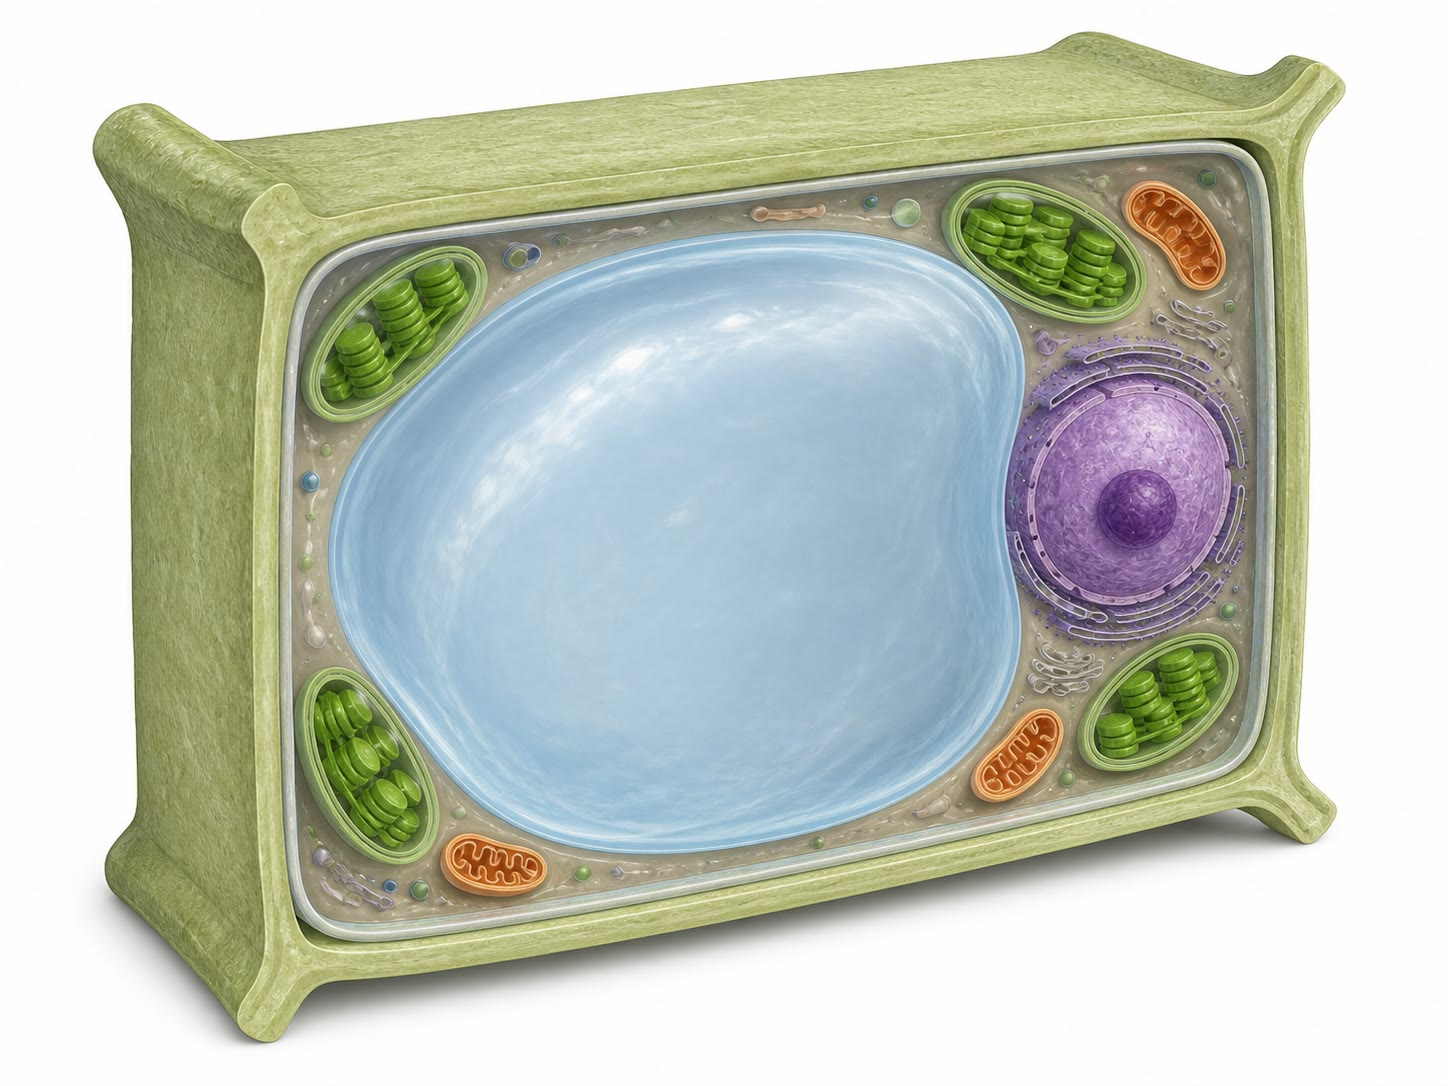
\includegraphics[width=0.52\linewidth]{images/book2/ai/fig-plant-cell-cutaway-v2.jpg}};
  \begin{scope}[x={(img.south east)}, y={(img.north west)},
      every node/.style={font=\small}]
    \draw[omDef, thick] (0.50,0.50) -- (0.50,1.08) node[above] {centrale vacuole};
    \draw[omDef, thick] (0.10,0.50) -- (-0.03,0.56) node[left] {celwand};
    \draw[omDef, thick] (0.25,0.73) -- (-0.03,0.84) node[left] {chloroplast};
    \draw[omDef, thick] (0.35,0.17) -- (-0.03,0.12) node[left] {mitochondrion};
    \draw[omDef, thick] (0.76,0.47) -- (1.03,0.60) node[right] {celkern};
    \draw[omDef, thick] (0.60,0.13) -- (1.03,0.16) node[right] {dun cytoplasma};
  \end{scope}
\end{tikzpicture}

{\small Een plantencel: de wand buiten de membraan, de \omterm{def:b1:eukaryotic-cell:plantcell}{vacuole} die het grootste
deel van het volume vult, \omterm{def:b1:eukaryotic-cell:plastid}{chloroplasten} en \omterm{def:b1:eukaryotic-cell:mitochondrion}{mitochondriën} in de dunne laag
\omterm{def:b1:cell-unit-of-life:cell}{cytoplasma} daartussen.}
\end{omfigure}

\begin{proposition}[Plantencel en dierlijke cel vergeleken]\label{prop:b1:eukaryotic-cell:compare}
Beide hebben een \omterm{def:b1:eukaryotic-cell:nucleus}{celkern}, ER, \omterm{def:b1:eukaryotic-cell:endomembrane}{golgi-apparaat}, \omterm{def:b1:eukaryotic-cell:mitochondrion}{mitochondriën}, \omterm{def:b1:eukaryotic-cell:peroxisome}{peroxisomen},
ribosomen en een \omterm{def:b1:eukaryotic-cell:cytoskeleton}{cytoskelet}. De plantencel heeft een cellulosewand, een grote
\omterm{def:b1:eukaryotic-cell:plantcell}{vacuole}, \omterm{def:b1:eukaryotic-cell:plastid}{plastiden} en plasmodesmata, en geen centriolen of \omterm{def:b1:eukaryotic-cell:endomembrane}{lysosomen} (de \omterm{def:b1:eukaryotic-cell:plantcell}{vacuole}
verteert); zij kruipt niet en slokt niet op, en deelt door dwars door het midden
een nieuwe wand te bouwen. De dierlijke \omterm{def:b1:cell-unit-of-life:cell}{cel} heeft geen wand (en kan dus van vorm
veranderen, kruipen en fagocyteren), wel \omterm{def:b1:eukaryotic-cell:endomembrane}{lysosomen} en een \omterm{def:b1:eukaryotic-cell:cytoskeleton}{centrosoom} met
centriolen, en communiceert via \omterm{def:b1:body-plans-tissues:epithelium}{celverbindingen} in plaats van plasmodesmata; zij
deelt door zich in tweeën te snoeren.
\end{proposition}

\begin{example}[Turgor]\label{ex:b1:eukaryotic-cell:turgor}
Een bladcel waarvan de \omterm{def:b1:eukaryotic-cell:plantcell}{vacuole} \qty{0.3}{mol/L} opgeloste stoffen bevat, trekt
water aan tot de wand met een druk van ongeveer \qty{0.7}{MPa} terugduwt, zeven
atmosfeer; de \omterm{def:b1:cell-unit-of-life:cell}{cel} is dan turgescent en het \omterm{def:b1:flowering-plant-organization:organs}{blad} stevig. Ontnomen van water
verliest de \omterm{def:b1:eukaryotic-cell:plantcell}{vacuole} volume, daalt de druk tot nul, en verwelkt het \omterm{def:b1:flowering-plant-organization:organs}{blad} --- de
wand onveranderd, de druk verdwenen
(\cref{ch:b1:membranes-transport}). Een dierlijke \omterm{def:b1:cell-unit-of-life:cell}{cel} in dezelfde oplossing zou,
zonder wand, eenvoudigweg barsten.
\end{example}

\section{Opgaven}

\begin{exercise}[$\star$]\label{exo:b1:eukaryotic-cell:1}
Noem de door membranen begrensde \omterm{def:b1:cell-unit-of-life:prokeuk}{organellen} van een dierlijke \omterm{def:b1:cell-unit-of-life:cell}{cel} en geef in
enkele woorden van elk de belangrijkste functie.
\end{exercise}

\begin{exercise}[$\star$]\label{exo:b1:eukaryotic-cell:2}
Volg de weg van een verteringsenzym van zijn synthese tot de afvoerbuis, en noem
elk compartiment en de manier waarop het eiwit ertussen passeert.
\end{exercise}

\begin{exercise}[$\star$]\label{exo:b1:eukaryotic-cell:3}
Welk deel van het membraan van de \omterm{def:b1:cell-unit-of-life:cell}{cel} is volgens de figuur van de membraanbalans
mitochondriaal (buiten plus binnen)? Waarom is het binnenmembraan zoveel groter
dan het buitenmembraan?
\end{exercise}

\begin{exercise}[$\star$]\label{exo:b1:eukaryotic-cell:4}
Geef drie structuren die een plantencel heeft en een dierlijke \omterm{def:b1:cell-unit-of-life:cell}{cel} niet, en twee
die de dierlijke \omterm{def:b1:cell-unit-of-life:cell}{cel} heeft en de plantencel niet.
\end{exercise}

\begin{exercise}[$\star\star$]\label{exo:b1:eukaryotic-cell:5}
Op welk tijdstip piekt het merk volgens de figuur van de puls-jachtproef in het
ER, in het \omterm{def:b1:eukaryotic-cell:endomembrane}{golgi-apparaat} en in de korrels? Schat de transporttijd van ER naar
korrel en de tijd tot de helft van het merk is afgescheiden.
\end{exercise}

\begin{exercise}[$\star\star$]\label{exo:b1:eukaryotic-cell:6}
Een \omterm{def:b1:cell-unit-of-life:cell}{cel} wordt behandeld met een middel dat \omterm{def:b1:eukaryotic-cell:cytoskeleton}{microtubuli} afbreekt. Voorspel de
gevolgen voor de plaats van het \omterm{def:b1:eukaryotic-cell:endomembrane}{golgi-apparaat}, voor het blaasjesverkeer, voor
de celdeling en voor het slaan van trilharen.
\end{exercise}

\begin{exercise}[$\star\star$]\label{exo:b1:eukaryotic-cell:7}
Geef vier stukken bewijsmateriaal voor de bacteriële oorsprong van \omterm{def:b1:eukaryotic-cell:mitochondrion}{mitochondriën},
en leg uit waarom een \omterm{def:b1:eukaryotic-cell:mitochondrion}{mitochondrion} desondanks niet buiten een \omterm{def:b1:cell-unit-of-life:cell}{cel} kan leven.
\end{exercise}

\begin{exercise}[$\star\star$]\label{exo:b1:eukaryotic-cell:8}
Het lumen van het ER is ``topologisch buiten de \omterm{def:b1:cell-unit-of-life:cell}{cel}''. Verklaar die uitdrukking
door een membraaneiwit waarvan de suikerketens naar het lumen wijzen van het ER
naar de plasmamembraan te volgen: naar welke kant wijzen de suikers aan het eind?
\end{exercise}

\begin{exercise}[$\star\star$]\label{exo:b1:eukaryotic-cell:9}
Een afscheidende \omterm{def:b1:cell-unit-of-life:cell}{cel} geeft per dag \qty{2000}{} korrels van \qty{1}{\micro m}
doorsnede af via een apicaal oppervlak van \qty{40}{\micro m^2}. Bereken het
membraan dat per dag wordt aangevoerd en hoe vaak het apicale oppervlak moet
worden hergebruikt. Wat betekent dat?
\end{exercise}

\begin{exercise}[$\star\star\star$]\label{exo:b1:eukaryotic-cell:10}
In een reageerbuis met ribosomen, mRNA voor een secretie-eiwit en aminozuren is
het product een keten van \qty{320}{} residuen; met ER-blaasjes erbij verschijnt
er binnen de blaasjes een keten van \qty{300}{} residuen die niet door een
naderhand toegevoegd protease wordt verteerd. Duid elke waarneming, en zeg wat
een mutant zonder de eerste twintig residuen zou doen.
\end{exercise}

\begin{exercise}[$\star\star\star$]\label{exo:b1:eukaryotic-cell:11}
De \omterm{def:b1:cell-unit-of-life:cell}{cellen} van een patiënt missen een lysosomaal enzym dat een lipide afbreekt;
de lipide hoopt zich op in gezwollen \omterm{def:b1:eukaryotic-cell:endomembrane}{lysosomen} en de \omterm{def:b1:cell-unit-of-life:cell}{cellen} sterven. Leg de
celbiologie uit, zeg waarom de ziekte het ergst is in \omterm{def:b1:cell-unit-of-life:cell}{cellen} die hun membranen
het snelst vernieuwen, en stel voor hoe een in het bloed gespoten enzym de
\omterm{def:b1:eukaryotic-cell:endomembrane}{lysosomen} zou kunnen bereiken.
\end{exercise}

\begin{exercise}[$\star\star\star$]\label{exo:b1:eukaryotic-cell:12}
``De \omterm{def:b1:cell-unit-of-life:prokeuk}{eukaryote cel} is een federatie van voormalige bacteriën, bijeengehouden door
een membraanstelsel.'' Bespreek dat in een alinea en weeg af wat de
endosymbiontentheorie verklaart tegen wat zij niet verklaart (\omterm{def:b1:eukaryotic-cell:nucleus}{celkern}, ER,
\omterm{def:b1:eukaryotic-cell:cytoskeleton}{cytoskelet}).
\end{exercise}

\section{Vraagstuk: de acinaire cel van de alvleesklier}

\begin{problem}[{Weekendvraagstuk --- een cel die elke dag haar eigen massa aan
eiwit afscheidt: de klok van Palade, het membraan dat zij moet hergebruiken, het
signaal dat het eiwit zijn route wijst, eindigend op de transporttijd van een
verteringsenzym}]
\label{pb:b1:eukaryotic-cell:1}
Een acinaire \omterm{def:b1:cell-unit-of-life:cell}{cel} van de alvleesklier is een kubus met ribbe \qty{12}{\micro m},
met haar apicale zijde (\qty{144}{\micro m^2}, aan de afvoerbuis) en haar basale
zijde aan het bloed. Een menselijke alvleesklier van \qty{80}{g} bevat ongeveer
$\num{8e10}$ van zulke \omterm{def:b1:cell-unit-of-life:cell}{cellen} en scheidt per dag \qty{10}{g} enzymeiwit af. Een
secretiekorrel is een bol van \qty{1}{\micro m} doorsnede met eiwit bij
\qty{200}{mg/mL}. Ribosomen voegen \qty{5}{} aminozuren per seconde toe; een
gebruikelijk enzym telt \qty{250}{} residuen met een gemiddelde massa van
\qty{110}{g/mol}.

\medskip
\noindent\textbf{Deel I --- De klok van Palade.}
De figuur van de puls-jachtproef uit het hoofdstuk geeft de plaats van het merk in
de tijd.
\begin{enumerate}
  \item Waarom moet de puls kort zijn en de jacht een grote overmaat
        ongemerkt aminozuur bevatten?
  \item Lees het tijdstip af waarop het merk piekt in het ER, in het
        \omterm{def:b1:eukaryotic-cell:endomembrane}{golgi-apparaat} en in de korrels.
  \item Schat de transporttijd van ER naar \omterm{def:b1:eukaryotic-cell:endomembrane}{golgi-apparaat} en van
        \omterm{def:b1:eukaryotic-cell:endomembrane}{golgi-apparaat} naar korrel.
  \item Waar zit het merk na \qty{60}{min}, en waarom heeft een deel de \omterm{def:b1:cell-unit-of-life:cell}{cel}
        al verlaten terwijl het meeste nog in korrels zit?
  \item Een tweede proef wordt bij \qty{15}{\celsius} gedaan: het merk
        blijft ruim een uur in het ER. Duid dat.
\end{enumerate}

\medskip
\noindent\textbf{Deel II --- De massa eiwit.}
\begin{enumerate}[resume]
  \item Bereken het per \omterm{def:b1:cell-unit-of-life:cell}{cel} per dag afgescheiden eiwit, in picogram.
  \item Bereken het volume van één korrel en de massa eiwit die zij bevat.
  \item Bereken het aantal korrels dat per \omterm{def:b1:cell-unit-of-life:cell}{cel} per dag en per minuut wordt
        vrijgegeven.
  \item Bereken het volume van de \omterm{def:b1:cell-unit-of-life:cell}{cel} en, met een dichtheid van
        \qty{1.05}{g/cm^3}, haar massa. Welk deel van haar eigen massa
        scheidt zij elke dag af?
  \item Bereken het aantal enzymmoleculen in één korrel (het getal van
        Avogadro $\num{6.0e23}$).
  \item Bereken de tijd die een ribosoom nodig heeft om één enzymmolecuul
        te maken.
  \item Hoeveel ribosomen moeten onafgebroken werken om de dagelijkse
        productie te halen? Vergelijk dat met de $\num{4e6}$ ribosomen die
        zo'n \omterm{def:b1:cell-unit-of-life:cell}{cel} bevat.
\end{enumerate}

\medskip
\noindent\textbf{Deel III --- Membraan.}
\begin{enumerate}[resume]
  \item Bereken het membraanoppervlak van één korrel.
  \item Bereken het membraan dat per dag door exocytose van de korrels uit
        vraag 8 aan de apicale zijde wordt aangevoerd.
  \item Hoe vaak per dag wordt het oppervlak van de apicale zijde
        toegevoegd? Wat moet de \omterm{def:b1:cell-unit-of-life:cell}{cel} ermee doen, en via welk proces?
  \item Het korrelmembraan komt van het \omterm{def:b1:eukaryotic-cell:endomembrane}{golgi-apparaat}, dat het van het ER
        krijgt. Als het ER van de \omterm{def:b1:cell-unit-of-life:cell}{cel} \qty{20000}{\micro m^2} membraan
        heeft, hoeveel dagen korrelmembraan is dat dan? Wat zegt dat over
        het hergebruik binnen het \omterm{def:b1:eukaryotic-cell:endomembrane}{endomembraansysteem}?
  \item De apicale zijde draagt \qty{2000}{} microvilli van
        \qty{0.1}{\micro m} doorsnede en \qty{1}{\micro m} lang. Met welke
        factor vergroten zij de \qty{144}{\micro m^2} van die zijde?
\end{enumerate}

\medskip
\noindent\textbf{Deel IV --- Het adres op het eiwit.}
\begin{enumerate}[resume]
  \item Het mRNA van een enzym, in een reageerbuis zonder membranen
        vertaald, geeft een keten die \qty{20}{} residuen langer is dan het
        enzym in de korrels. Waar zitten de extra residuen en wat zijn zij?
  \item Met ER-blaasjes erbij heeft het product de juiste lengte, zit het
        binnen de blaasjes, en is het tegen een protease beschermd. Duid
        dat.
  \item Dezelfde proef met het mRNA van een cytosolisch enzym geeft een
        product buiten de blaasjes dat niet beschermd is. Trek een
        conclusie.
  \item Een mutatie verwijdert de twintig residuen. Voorspel waar het enzym
        terechtkomt en wat er met de \omterm{def:b1:cell-unit-of-life:cell}{cel} gebeurt.
  \item Een ander enzym wordt in de \omterm{def:b1:eukaryotic-cell:endomembrane}{lysosomen} gevonden in plaats van in de
        korrels. Het draagt hetzelfde soort \omterm{prop:b1:eukaryotic-cell:secretory}{signaalsequentie}. Waar langs
        de route moet de tweede beslissing worden genomen, en in grote
        lijnen door welk mechanisme?
  \item Een \omterm{def:b1:cell-unit-of-life:cell}{cel} wordt behandeld met een middel dat de ATP-synthese
        blokkeert. Voorspel waar het merk van een puls-jachtproef zich
        ophoopt en waarom (twee redenen).
  \item Combineer de vragen 3 en 8: hoeveel korrels zijn er in een
        stationaire toestand op elk moment ``onderweg'' tussen ER en
        korrel?
  \item Vat het resultaat samen: de transporttijd van synthese tot korrel,
        de tijd tot afscheiding, het aantal korrels per minuut, en het deel
        van haar eigen massa dat de \omterm{def:b1:cell-unit-of-life:cell}{cel} dagelijks afscheidt.
\end{enumerate}
\end{problem}
